\documentclass[11pt,
			   %10pt, 
               %hyperref={colorlinks},
               aspectratio=169
               ]{beamer}
\usetheme{Singapore}
\usecolortheme[snowy]{owl}

\usepackage[utf8]{inputenc}
\usepackage[T1]{fontenc}
\usepackage[american]{babel}
\usepackage{graphicx}
\usepackage{hyperref}

\usepackage[natbib=true,style=authoryear,backend=bibtex,useprefix=true]{biblatex}
%\setbeamercolor*{bibliography entry title}{fg=black}
%\setbeamercolor*{bibliography entry location}{fg=black}
%\setbeamercolor*{bibliography entry note}{fg=black}
\definecolor{OwlGreen}{RGB}{75,0,130} % easier to see
\setbeamertemplate{bibliography item}{}
\setbeamerfont{caption}{size=\footnotesize}
\setbeamertemplate{frametitle continuation}{}
\renewcommand*{\bibfont}{\scriptsize}


\author{Patrick Hall}
\title{Affecting Change with Data}
\subtitle{A Primer on Hype and Reality in Data Mining}
\institute{\href{https://www.h2o.ai}{H\textsubscript{2}O.ai}}
\date{July 26th, 2018}

% for nice quotes 
\usepackage{epigraph}
% \epigraphsize{\small}% Default
\setlength\epigraphwidth{14cm}
\setlength\epigraphrule{0pt}
\usepackage{etoolbox}
\makeatletter
\patchcmd{\epigraph}{\@epitext{#1}}{\itshape\@epitext{#1}}{}{}
\makeatother

% for newlines in tables
\usepackage{makecell}



\begin{document}
	
	\maketitle
	
	\begin{frame}
	
		\frametitle{Agenda}
	
		\tableofcontents{}
	
	\end{frame}

	\section*{Preface}

		\begin{frame}

			\frametitle{Preface}

			\epigraph{“We are drowning in information and starving for knowledge.”}{--- \textup{Rutherford Roger}, Librarian (1915 - 2015)}

			\epigraph{“Information is not knowledge. Knowledge is not wisdom. Wisdom is not truth. Truth is not beauty.”}{--- \textup{Frank Zappa}, Musician (1940 - 1993)}

			\epigraph{“All models are wrong, but some are useful.”}{--- \textup{George Box}, Statistician (1919 – 2013)}

		\end{frame}

	\section{Disambiguation}
	
		\subsection*{}
		
		\begin{frame}[t]
		
			\frametitle{Buzzword Disambiguation}
			
			\begin{figure}[htb]
				\begin{center}
					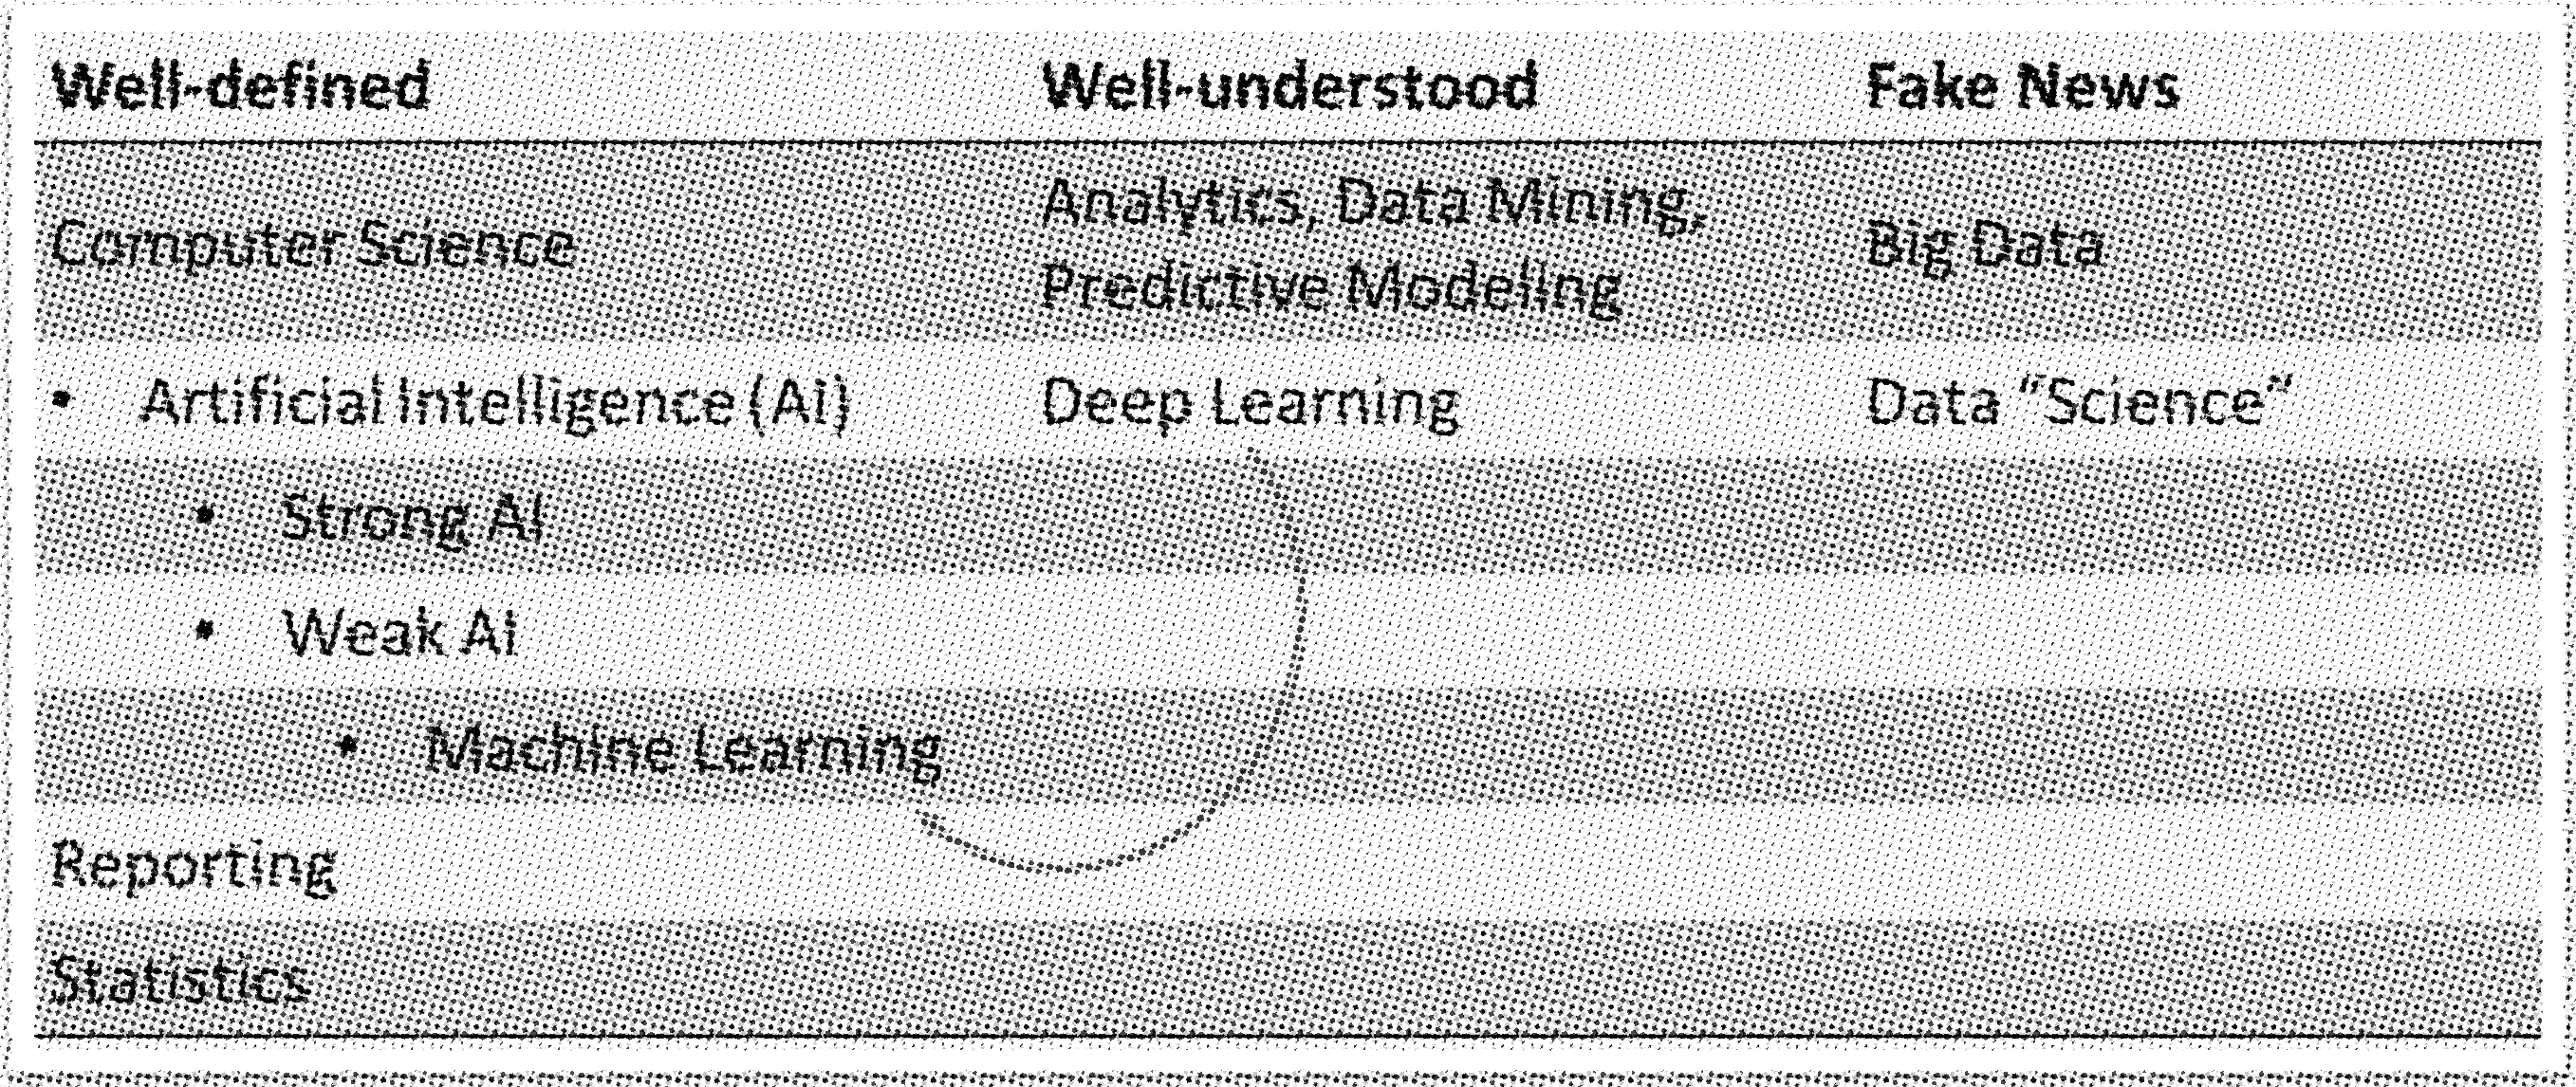
\includegraphics[height=155pt, angle=1]{img/buzzwords.png}
					\label{fig:buzzwords}
				\end{center}
			\end{figure}
		
		\end{frame}

		\begin{frame}
		
			\frametitle{Buzzword Disambiguation}
			
			\begin{figure}[htb]
				\begin{center}
					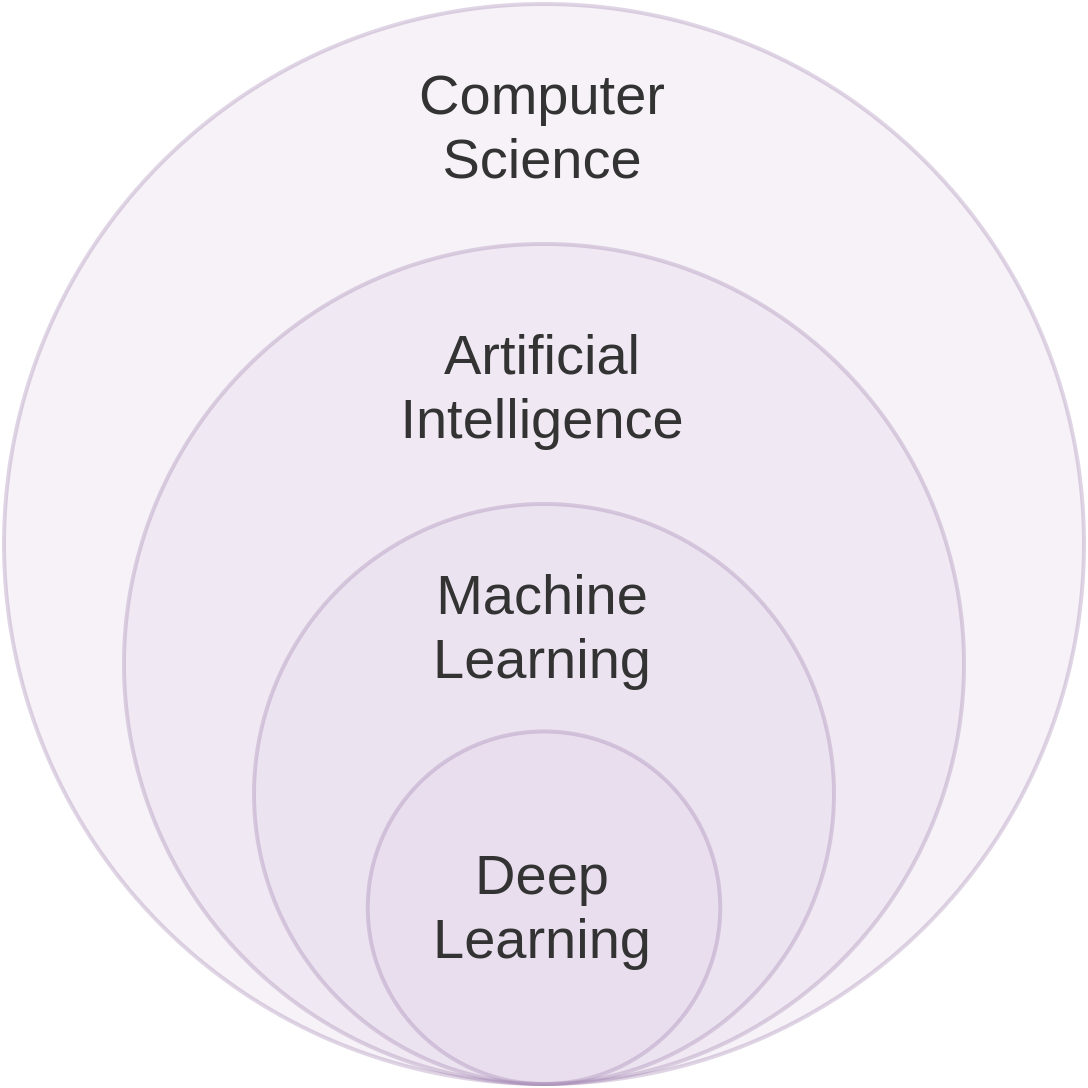
\includegraphics[height=165pt, angle=1]{img/cs.png}
					\label{fig:cs}
				\end{center}
			\end{figure}
		
		\end{frame}
			
		\begin{frame}
		
			\frametitle{Buzzword Disambiguation}
			
			\begin{figure}[htb]
				\begin{center}
					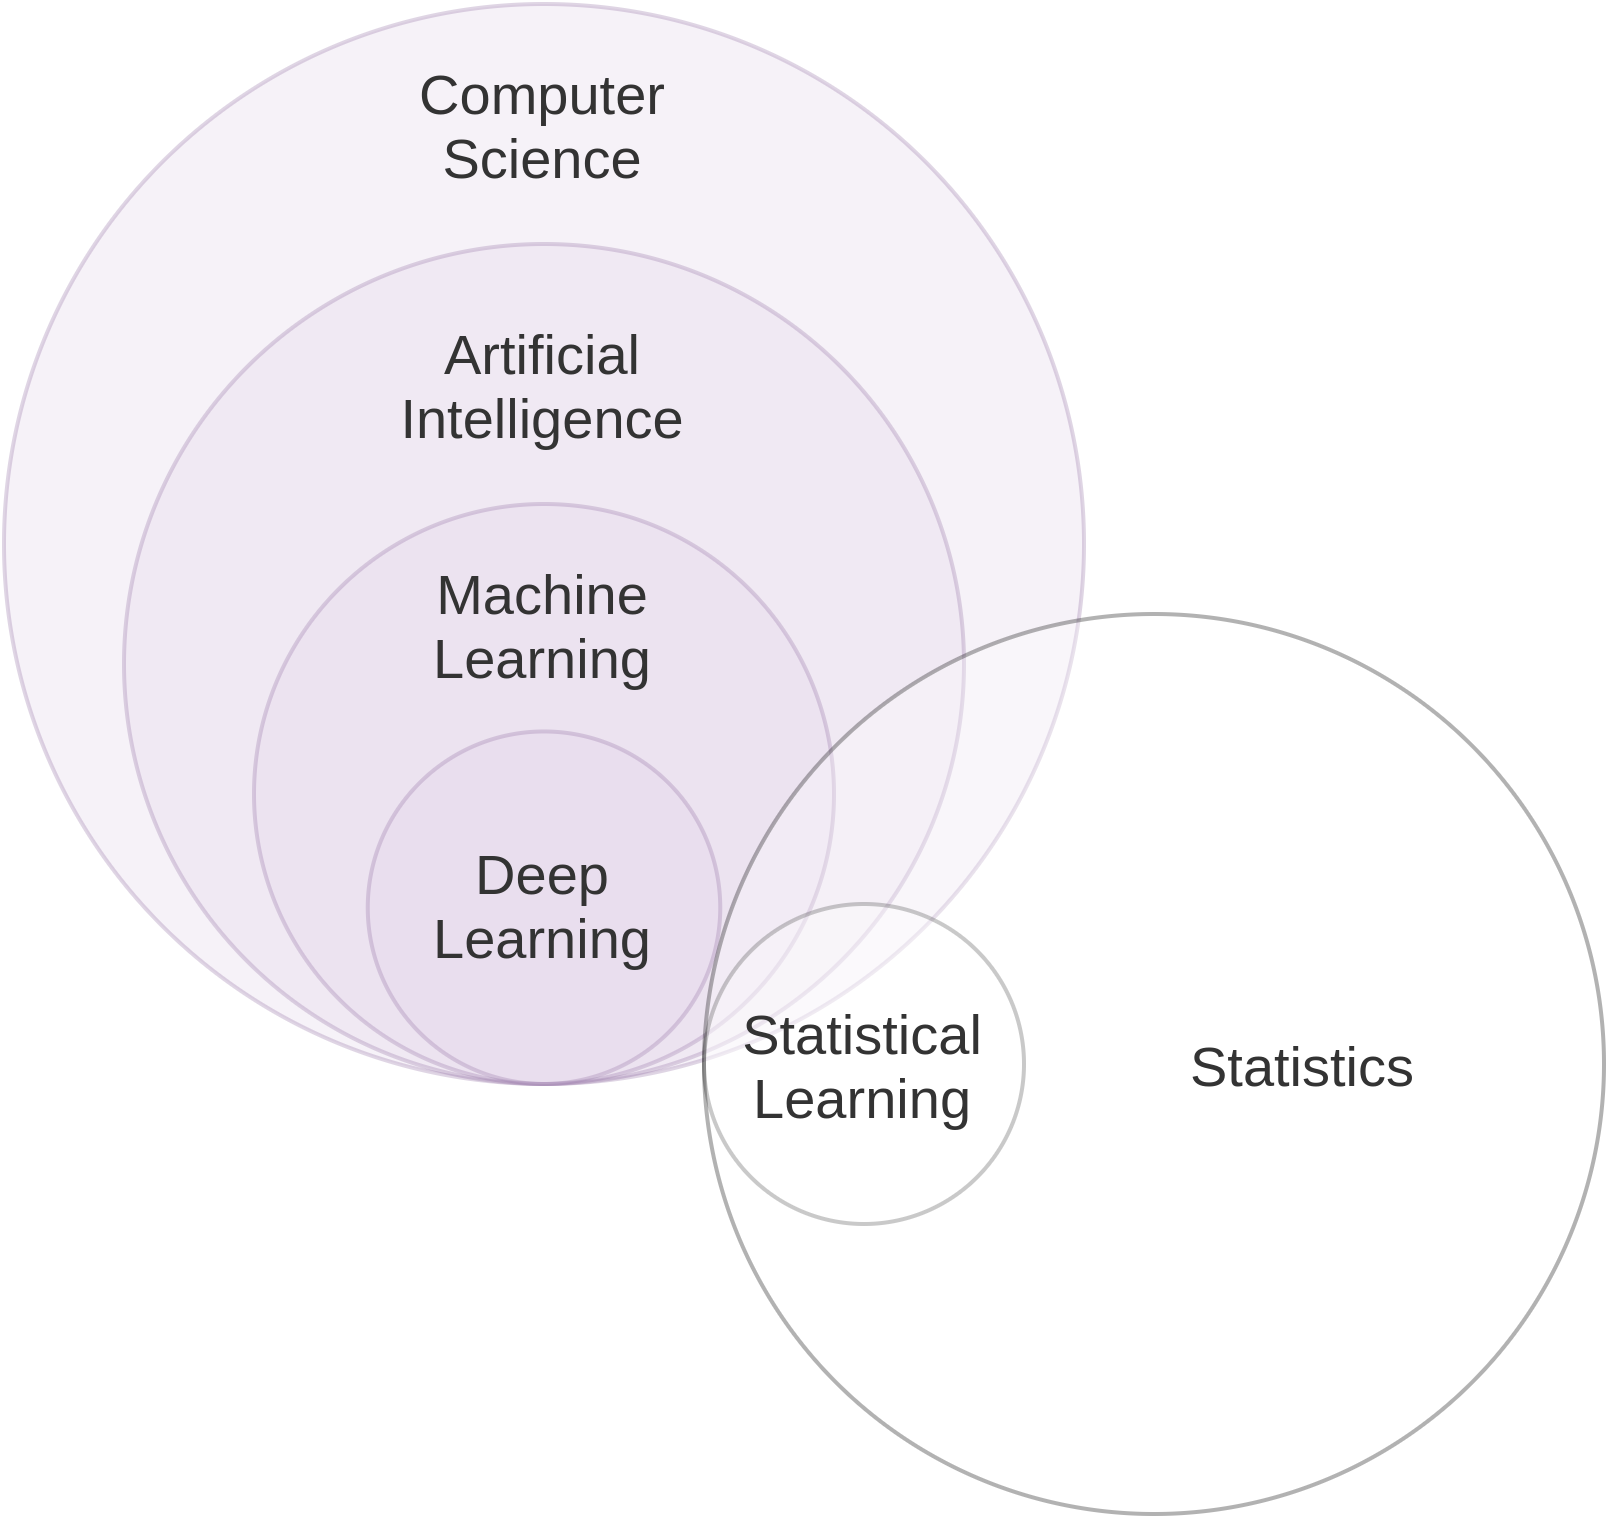
\includegraphics[height=165pt, angle=1]{img/cs_stat.png}
					\label{fig:cs}
				\end{center}
			\end{figure}
		
		\end{frame}
		
		\begin{frame}
		
			\frametitle{Buzzword Disambiguation}
			
			\begin{figure}[htb]
				\begin{center}
					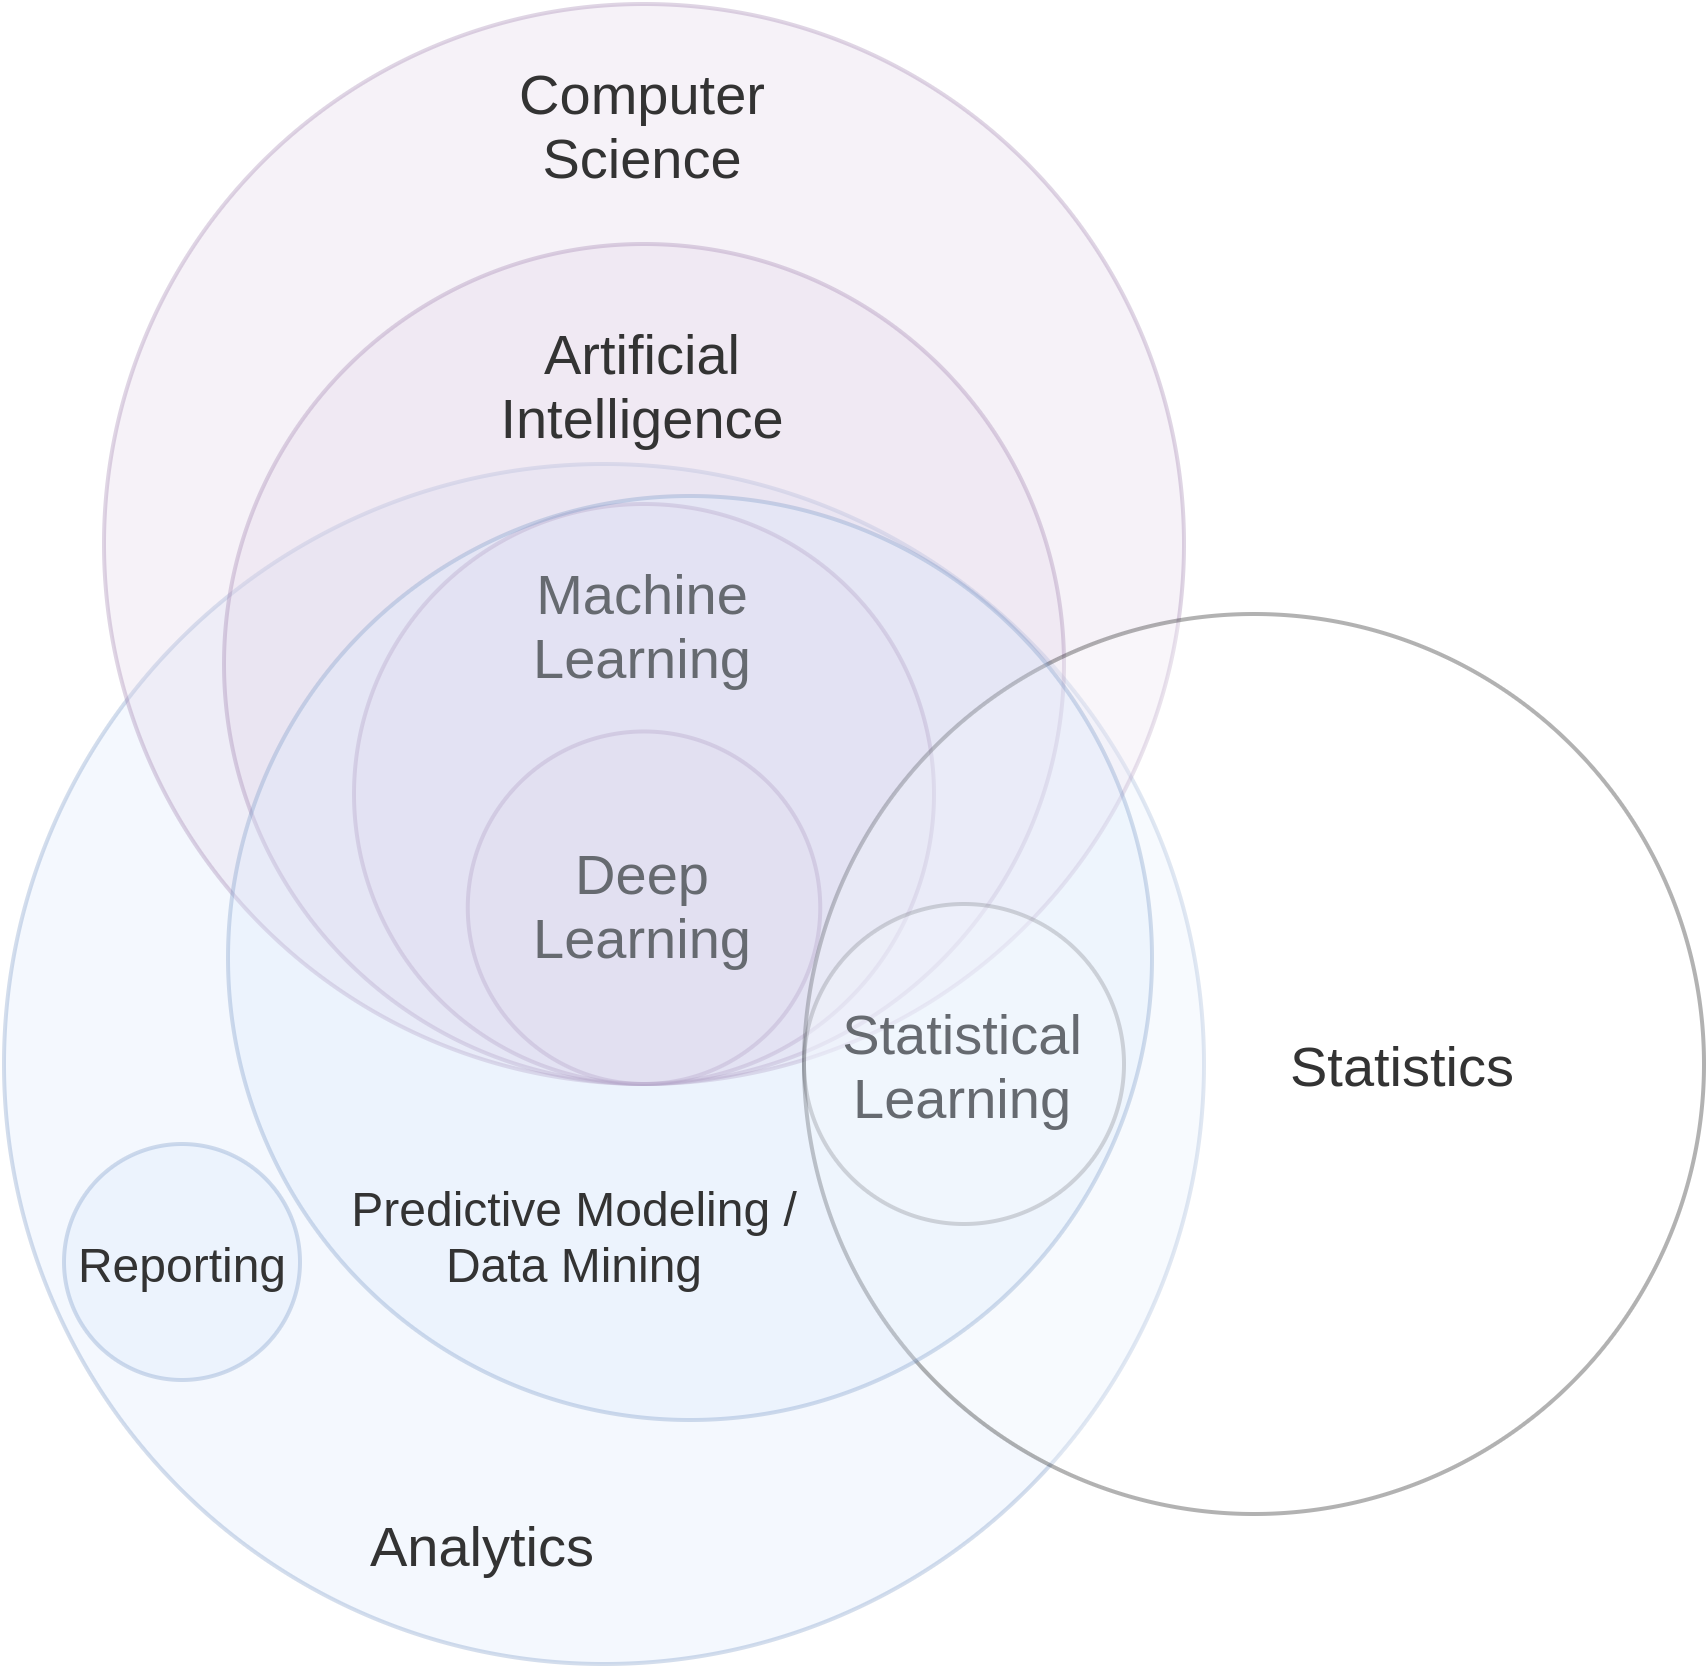
\includegraphics[height=165pt, angle=1]{img/cs_stat_an.png}
					\label{fig:cs}
				\end{center}
			\end{figure}
		
		\end{frame}
	
		\begin{frame}
		
			\frametitle{Buzzword Disambiguation}
			
			\begin{figure}[htb]
				\begin{center}
					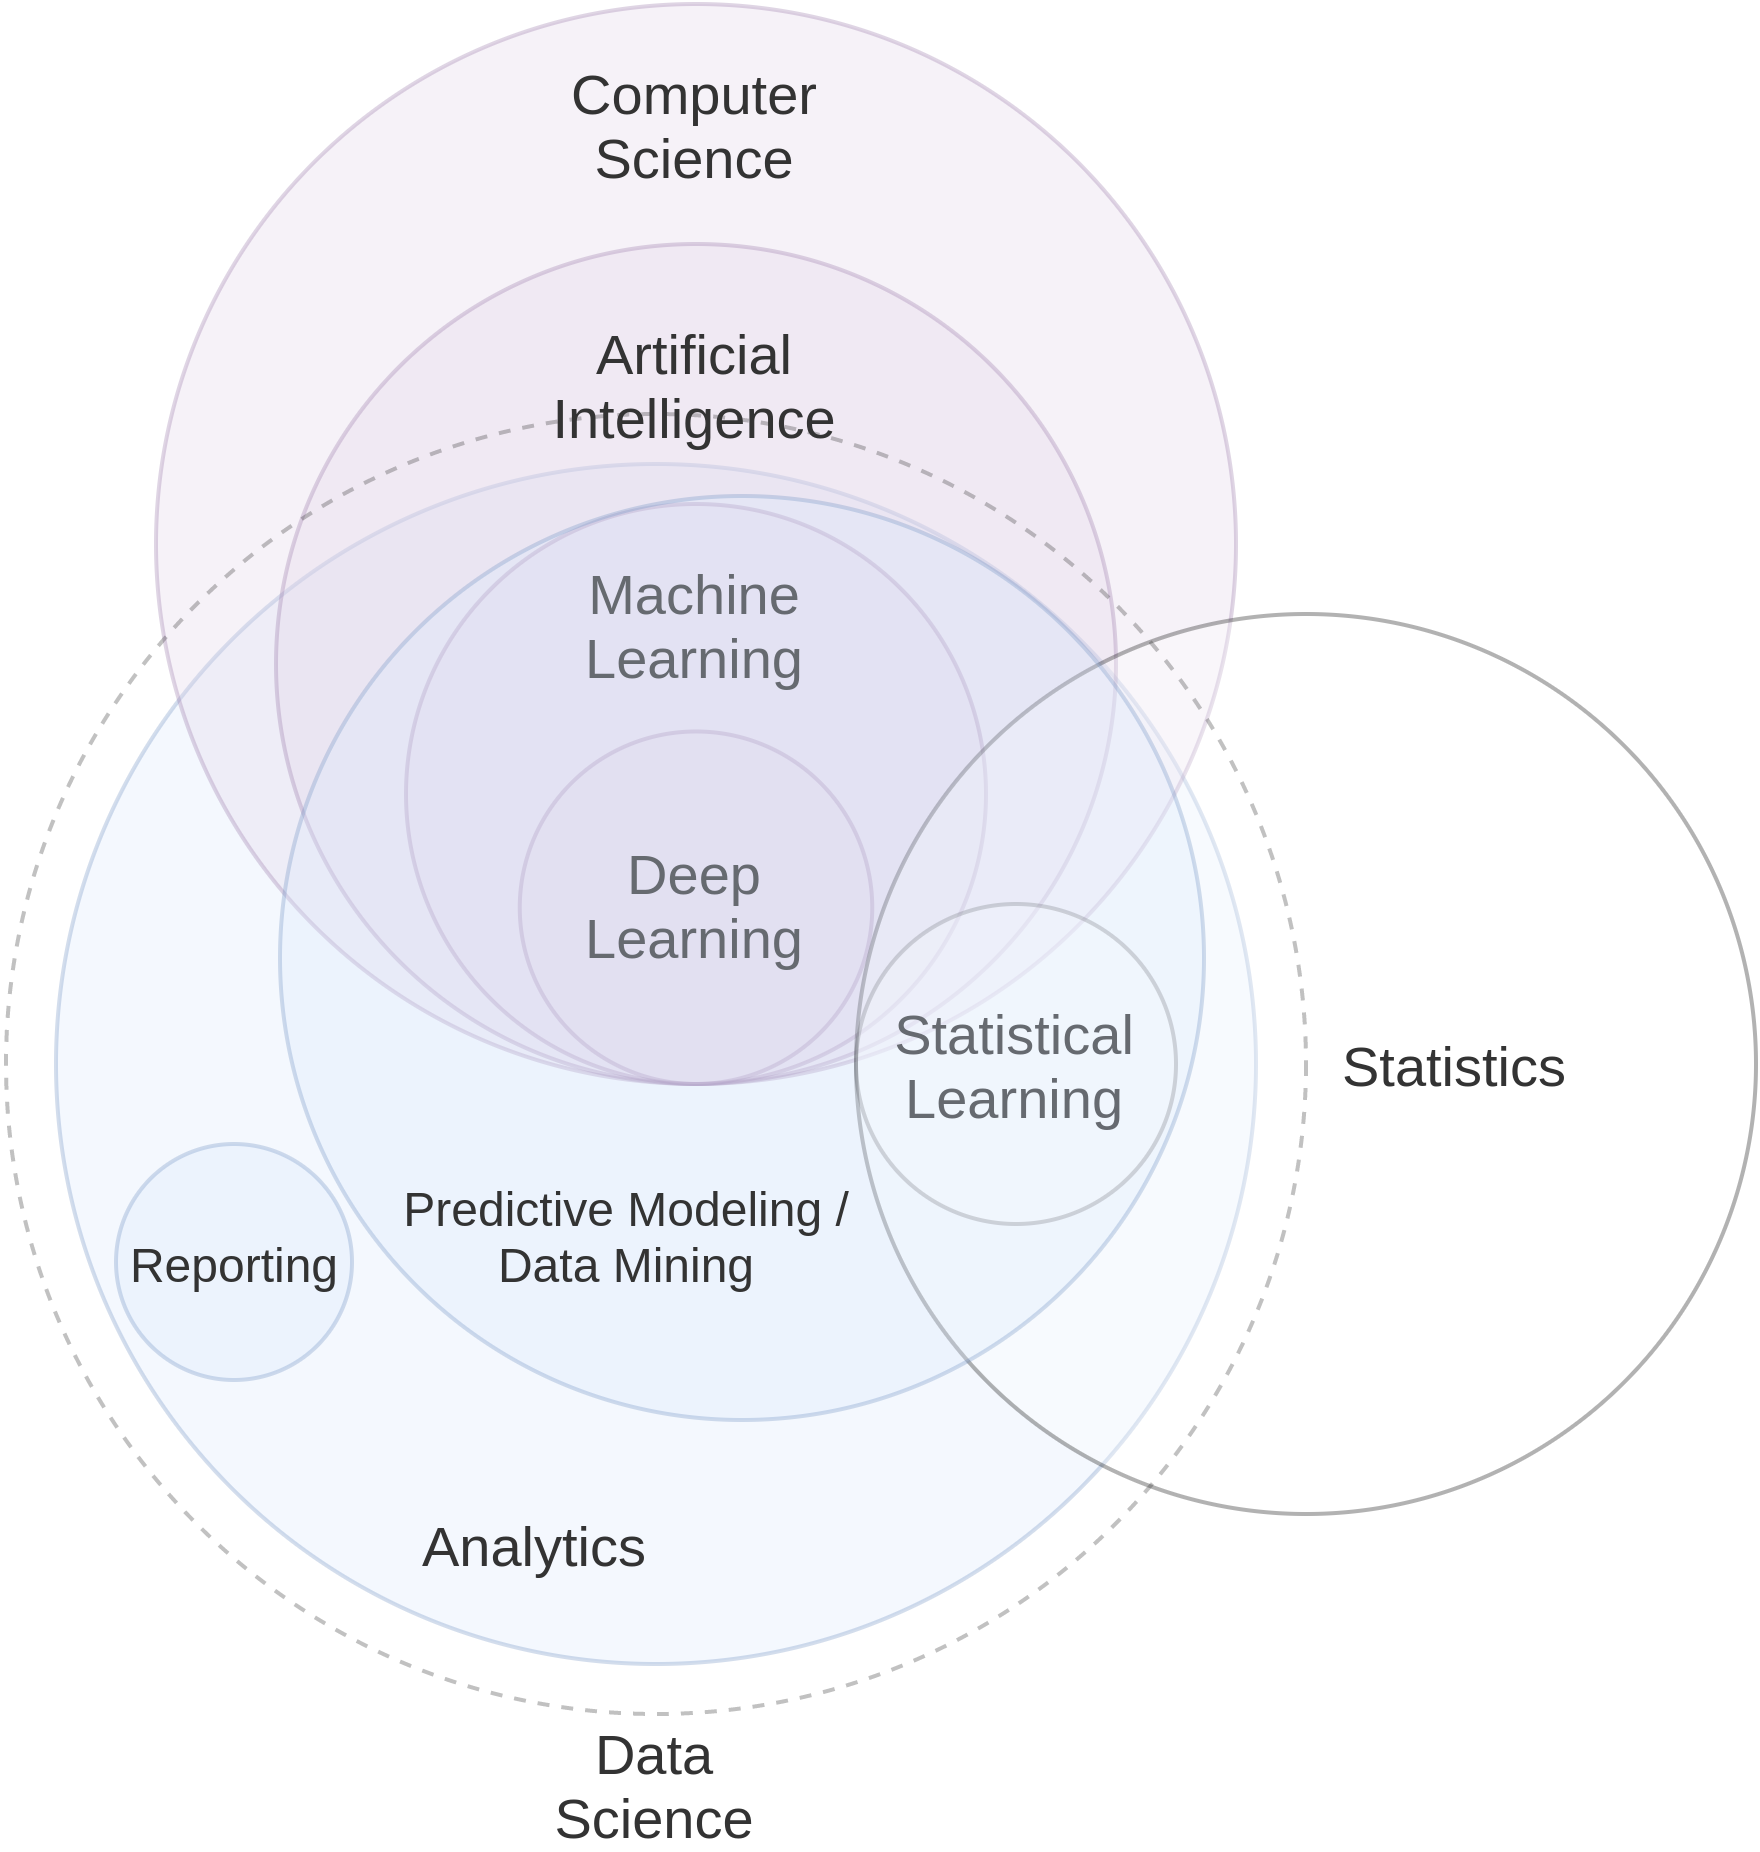
\includegraphics[height=165pt, angle=1]{img/cs_stat_an_ds.png}
					\label{fig:cs}
				\end{center}
			\end{figure}
		
		\end{frame}	
	
	
	\section{Hype and Reality}
	
		% There is nothing fundamentally new here, yet.
	
		\begin{frame}
		
			\frametitle{Hype and Reality}
	
			\begin{columns}
	
				\column{0.4\linewidth}
				\centering
				\includegraphics[height=110pt]{img/hype_reality.jpg}
	
				\column{0.6\linewidth}
				\vspace{-5pt}
				\begin{itemize}
					
					\item Data mining has been used for decades in traditional industries to improve financial margins.
					\item Big tech. made a windfall by overselling new but minor conveniences often at the cost of our personal privacy. 
					\item As usual, we \textit{may} be on the brink of a nonlinear leap in technology.
					
				\end{itemize}
				
	
			\end{columns}

			\vspace{10pt}

			\tiny Image credit: Shutterstock --- KimSongsak
			
			% https://www.shutterstock.com/image-photo/past-present-future-technology-devices-typewriter-391037419

		\end{frame}
		
	
	\section{Short History}
	
		\begin{frame}
	
			\frametitle{A Very Short History of Machine Learning}
	
				\begin{figure}[htb]
					\begin{center}
						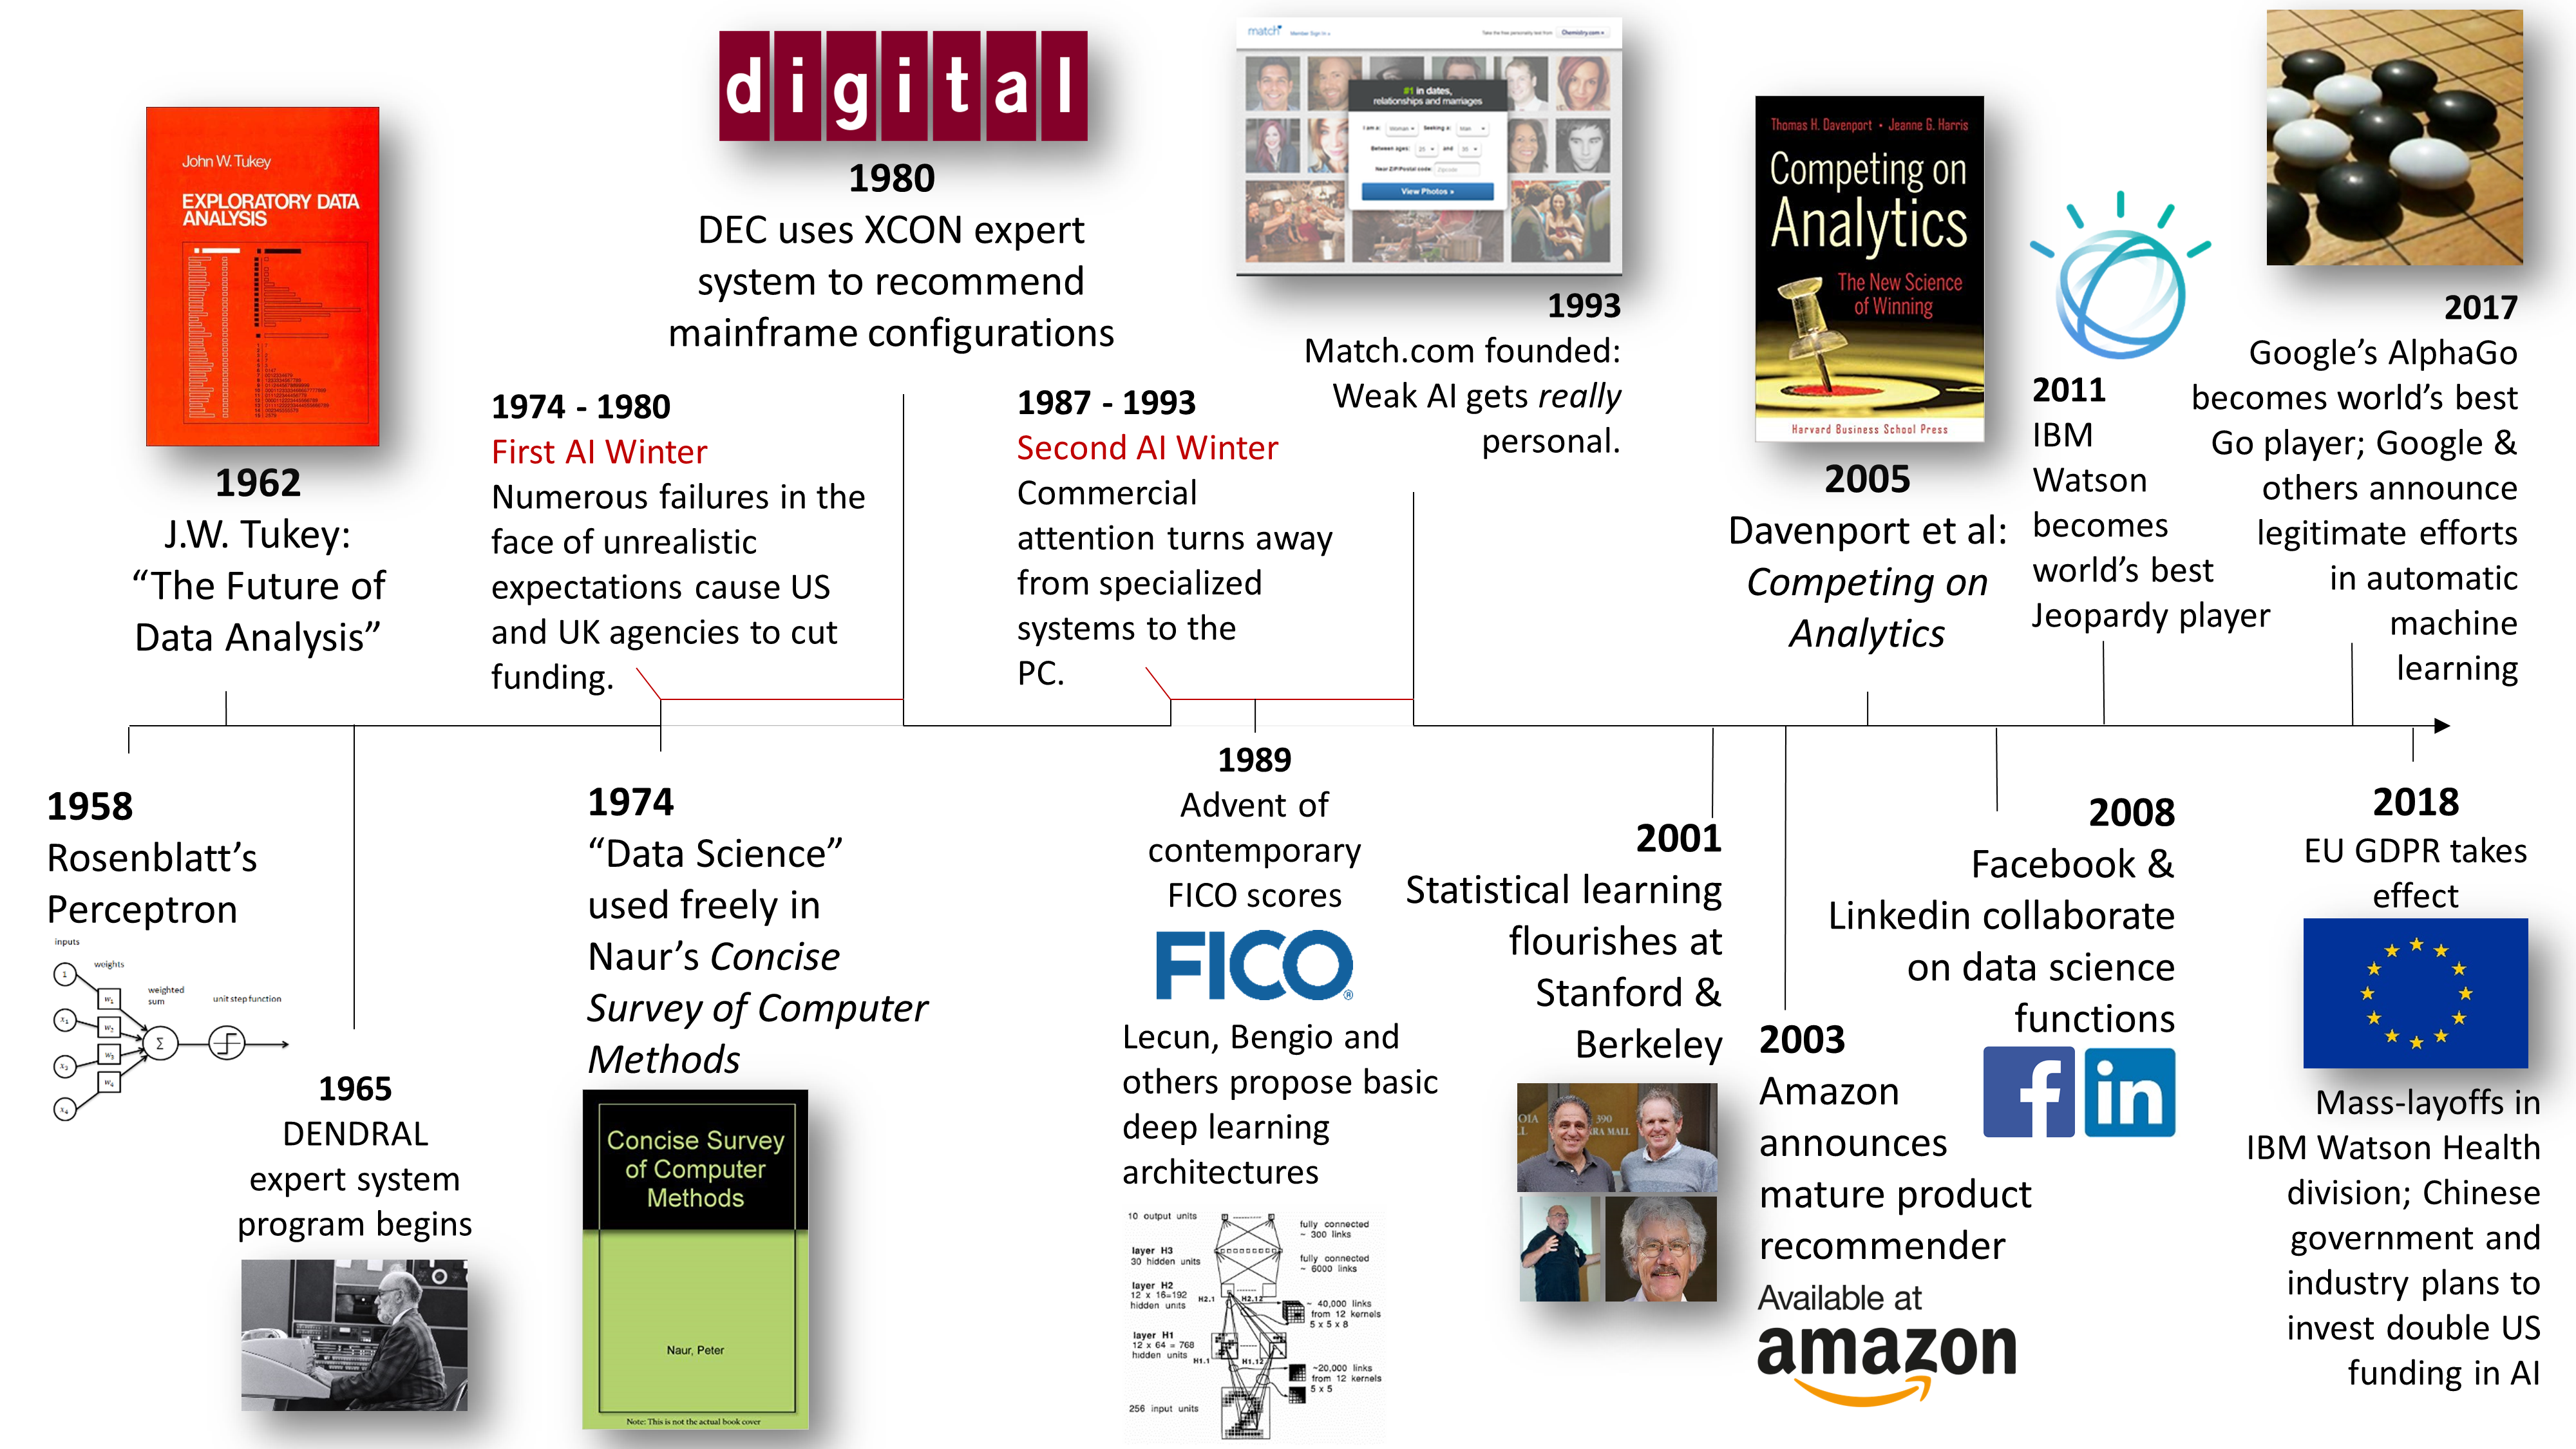
\includegraphics[height=185pt]{img/timeline.png}
						\label{fig:timeline}
					\end{center}
				\end{figure}
	
		\end{frame}	
	
	\section{Affecting Change}
	
		\begin{frame}[t]
		
			\frametitle{Affecting Change with Data}
		
			\vspace{-10pt}
		
			\begin{figure}[htb]
				\begin{center}
					\includegraphics[height=105pt]{img/past_present_future.png}
					\label{fig:pat_present_future}

				\end{center}
			\end{figure}
		
			\vspace{-20pt}
		
			Data mining is a blunt tool for revisiting the past, understanding the present, and seeing into the future.
			
			\vspace{10pt}
			
			\tiny Image credits: Flickr --- chengyee, Andy Castro, Roo Reynolds
			
			% https://www.flickr.com/photos/chengyee/253124450
			% https://www.flickr.com/photos/andycastro/2548898515
			% https://www.flickr.com/photos/rooreynolds/37305217
		
		\end{frame}
	
	\subsection{Past}
		
		\begin{frame}
		
			\frametitle{Learn from the Past}
		
			\begin{columns}
				
				\column{0.5\linewidth}
				\vspace{-15pt}
				\begin{itemize}
					\item Often easier to conduct as an individual as tangible results include papers, data visualizations, stories, lessons, and morals.
					\item Use common sense to learn about human or financial gain or loss.
					\item Look for trends, groups, and outliers in data.
				\end{itemize}

				\column{0.5\linewidth}
				\centering
				\includegraphics[height=140pt]{img/past.png}
				
				
	
			\end{columns}
		
			\tiny Image credit: Flickr --- David P. Whelan
			% https://www.flickr.com/photos/davidpwhelan/33418053762
		
		\end{frame}

	\subsection{Present}

		\begin{frame}
		
			\frametitle{Understand the Present}
		
			\begin{columns}
			
				\column{0.5\linewidth}
				\centering
				\includegraphics[height=140pt]{img/present.jpg}
			
				\column{0.45\linewidth}
					Typically requires organizational information technology (IT) support as tangible results include real-time reports and alerts created from data and IT systems.  
			\end{columns}
		
			\vspace{10pt}
		
			\tiny Image credit: Flickr --- Sérgio Bernardino
			% https://www.flickr.com/photos/smpb/4071022873
		
		\end{frame}	
		
	\subsection{Future}

		\begin{frame}
		
			\frametitle{Prepare for the Future}
			
			\begin{columns}
					
				\column{0.58\linewidth}
				\begin{itemize}
				\item Usually requires advanced IT support.
				\item Tangible results are typically decisions about customers, patients, students, equipment, or other valuable entities made by sophisticated computer systems.
				\item Common commercially viable applications include:
					\begin{itemize}
						\item Quantifying future risk
						\item Personalized promotions
						\item Predicting churn 
						\item Recommending products or content
					\end{itemize}
				\end{itemize}
				\column{0.4\linewidth}
				\centering
				\includegraphics[height=150pt, angle=-2]{img/future.png}
				
			\end{columns}
		
		\end{frame}		
				
	\section{Precautions}
		
		\begin{frame}
		
			\frametitle{Take Necessary Precautions}	
		
				\begin{columns}
					
					\column{0.38\linewidth}
						\centering
						\includegraphics[height=115pt]{img/surveillance.jpg}
					
					\column{0.58\linewidth}
					\begin{itemize}
						\item Data can be biased, incomplete, or just wrong.
						\item Results can be ignored or used politically.
						\item Avoid:
							\begin{itemize} 
								\item Confirmation bias 
								\item Testing multiple hypotheses   
								\item Unintended discrimination 
								\item Privacy violations
								\item Unmanageable complexity
							\end{itemize}
					\end{itemize}				
						
				\end{columns} 

				\vspace{10pt}

				\tiny Image credit: Flickr --- Thomas Hawk
				% https://www.flickr.com/photos/thomashawk/5318245724

		\end{frame}

	\section*{Stay in Touch}
	
		\begin{frame}
		
			\frametitle{Stay in Touch}
			
			\begin{tabular}{m{1.5cm} m{8cm}}
				
\includegraphics[height=40pt]{img/li.jpg} \newline &  
 				\href{https://www.linkedin.com/in/jpatrickhall}{linkedin.com/in/jpatrickhall} \newline \\
 				
\includegraphics[height=30pt]{img/twitter.png} &
 				\href{https://twitter.com/jpatrickhall}{@jpatrickhall}
			\end{tabular}

		\end{frame}

\end{document}